\section{\label{results}Results}


\subsection{\label{Hypotheses} Hypotheses}

We stress the fact that our investigation focuses on moving
pedestrians in a highly dense situation (say, the one experienced at
the Jamaraat bridge). As mentioned in Section \ref{introduction} , a deep
examination of the (basic) SFM parameters is required before
proceeding to any extension of the model.\\

Recall from the video analysis of the Muslim pilgrimage in Mina/Makkah
(see Section \ref{introduction}) that high-density flows can turn to a
temporarily interrupted flux, as people
start pushing to gain space \cite{helbing3}. This unexpected behavior can not be
reproduced by the (basic) SFM, seemingly because of ``an
underestimation of the local interactions triggered by high densities"
\cite{yu1}, or, the absence of a ``delayed reaction in cases of unexpected
behaviors" \cite{johansson}. Both statements are currently working hypotheses since
experimental data (specifically, measurements of pedestrian flux and
densities) does not ``provide any insight into the mechanisms and
dynamics behind the pedestrians interactions and behaviors" \cite{johansson}.\\

Researchers propose a ``re-calibration" of the (basic) SFM, in order to
attain ``stop-and-go" flows for highly dense crowds
\cite{yu1,johansson}. Presumably, this kind of instabilities within the crowd prevent
people from stopping at extremely high densities. The intended
``re-calibration" consist on either enhancing the (local) social
interactions or increasing the net-time headway (roughly, the
relaxation time) for the high density regime. Both extensions,
however, may not exclude other possibilities involving not only
individual motion, but collective (mass) motion \cite{helbing3}. Researchers
further point out that the relevance of physical contact in extremely
dense crowds may suppose a somewhat commonality with granular
media exists \cite{helbing3}.\\

We show that the
experimental data (say, the flux-density diagram) can be modeled under
quasi-stationary conditions in the high density regime. Our starting
point is the re-examination of the (basic) SFM. We hypothesize that two
control parameters, $\mathcal{A}$ and $\mathcal{K}$ (see appendix \ref{appendix_1}) may handle
the collective motion in dense crowds. We presume that physical contact is
a key feature in dense crowds, despite the fact that other issues may
also contribute to the flow reduction \cite{johansson1}. However, the latter could
be satisfactorily omitted in past research \cite{johansson}, and thus, we will not
attempt to introduce further extensions to the (basic) SFM for the
sake of simplicity.\\

The former ``re-calibrations" accomplish the socio-psychological
response of the crowd to ``gain more space" (by either enhancing local
interactions or performing a delayed reaction). We are aware that
crowds may respond differently in many situations (see Ref.~\cite{drury1}). Our working
hypothesis, however, does not focus on the crowd socio-psychological
response, but on the physical contact among pedestrians (and the
walls). The socio-psychological attitude of the pedestrians will be
assumed to remain fixed along the simulations (with the anxiety level
limited to $v_d=1\,$m/s). \\


Our investigation appears somewhat restricted to the (almost)
uni-direction flow inspired in the Muslim pilgrimage in Mina/Makkah.
This means that the following ``re-calibration" results hold for
corridor-like situations, and are not intended to be (automatically)
translated to bottleneck situations. Neither can be extended to other
boundary conditions (say, no limiting walls) since the boundary is a
key feature of collective motion. Nevertheless, our results accomplish
the available data on the Hajj pilgrimages \cite{helbing3,lohner1}.



\subsection{\label{fundamental_diagram} Fundamental diagram in the original model}

In this Section we present the results relating the local flow, velocity and density (\textit{i.e.} the fundamental diagram). The measurements were taken in the middle of the corridor using the definitions given in Eq.~(\ref{ec-v}), Eq.~(\ref{ec-flow}), and as shown in Fig.~\ref{corridor}. All the results shown here correspond to $R=1$~m (see Eq.~(\ref{ec-flow}) and Fig.~\ref{corridor}). We further varied $R$ until $R=3$, but no significant changes were observed. \\

Fig~\ref{fundamental_diagram_flow}, shows the fundamental diagram (flow vs. density) for different corridor widths. We can distinguish the two typical regimes of the fundamental diagram. In the free flow regime ($\rho < 5$), the flow increases linearly with the density, since collisions between pedestrians (and with the walls) are scarce. Pedestrians are able to achieve their desired velocity, leading to a flow that grows linearly with the density ($J \propto \rho$) until $\rho=5$. This behavior applies to all the analyzed corridor widths.\\

On the other hand, we have the congested branch  for $\rho > 5$. Here we face two different scenarios:

\begin{itemize}
\item[(i)] For narrow corridors (say $w < 10$) we can see that the flow reduces as the density increases. This resembles the traditional behavior of the fundamental diagram reported in the literature. 
\item[(ii)] For wide corridors (say $w > 15$) we see that the flow increases with density. This contradicts the typical behavior of the fundamental diagram.   
\end{itemize}

In the case of narrow corridors, both the simulated case and the empirical results converge to a constant flow value. It is remarkable that the system does not reach a freezing state such as the one reported in Refs.\cite{lin,kwak}. Recall that our simulations do not include any respect factor (see Ref.\cite{parisi2}), or changes in the net-time headway (Ref.\cite{helbing3}), or the urge to see an attraction (Ref.\cite{kwak}). We assume a well defined target and the same $v_d$ for all the pedestrians.\\

The inset in Fig.~\ref{fundamental_diagram_flow} corresponds to the empirical data from Helbing (\cite{helbing3}). at the entrance of the Jamaraat bridge (the corridor width was $w=22$~m). Notice that our simulated results corresponding to a $w=22$~m corridor, exhibit a different behavior along the congested regime. In the simulated case, the flow increases even for the greatest explored density. On the contrary, the empirical data exhibit a flow reduction for $\rho > 5$ until reaching a plateau for the highest explored density values.  \\

In order to fulfill the experimental fundamental diagram, it becomes necessary that the flow at the maximum explored density ($\rho_{max} = 9$) does not exceed the flow at $\rho = 5$ (upper bound). That is:  $J(\rho = 9) < J(\rho = 5)$. From the flow definition in Eq.~(\ref{ec-flow}) we can derive the bounding values.

\begin{align*} 
v(\rho_{max}) &< \frac{5v_d}{\rho_{max}} \leq \frac{5}{9} v_d \\
\end{align*}

As our desired velocity is fixed at $v_d = 1$~m/s, we conclude that the speed at the maximum density has to be bounded by $v(\rho_{max}) \lesssim  0.5$~m/s in order to satisfy the qualitative behavior of the (experimental) fundamental diagram reported in the literature.\\

The above reasoning is consistent with the speed-density results shown in Fig.~\ref{fundamental_diagram_speed}. As a visual guide we plotted $v=0.5$~m/s with a horizontal dashed line. The close examination of $\rho_{max} = 9$ shows that values corresponding to the wide corridors ($w=15$~m and $w=22$~m) exceed $v=0.5$~m/s. But, those values corresponding to narrow corridors fall below $v=0.5$~m/s. \\

\begin{figure}[htbp!]
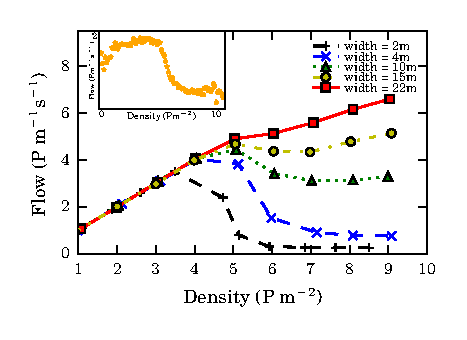
\includegraphics[width=0.5\columnwidth]
{plots/flow-density_vd1_multiple_widths.eps}
\caption{\label{fundamental_diagram_flow} Mean flow ($J$) as a function of the density ($\rho$) for different widths. Initially, 
pedestrians were randomly distributed along the corridor. The measurements were taken in the middle
of the corridor once the system reached the stationary state (see Fig.~\ref{corridor}). The length of the corridor 
was $L=$28~m for all cases (with periodic boundary conditions in the \textit{x} direction).}
\end{figure}

The results shown in Fig.~\ref{fundamental_diagram_speed} confirm the fact that when the density is low enough, pedestrians manage to walk at the desired velocity ($v=v_d=1$~m/s). Above $\rho>5$, however, the velocity begins to slow down. The inset shows the experimental data at the entrance of the Jamaraat bridge. We may conclude that our simulations agree with the experimental data for narrow corridors, but disagree as these become wider. The wider the corridor, the greater the velocity for all the density values explored. In Section \ref{velocity_profile} we will further discuss this topic.\\

It should be pointed out that the Jamaraat data does not a exhibit a ``really" constant velocity for low densities. But this seems reasonable since our simulations do not include the complexities of the real situation when the density is low. We will not analyze this phenomenon in this investigation. \\

\begin{figure}[htbp!]
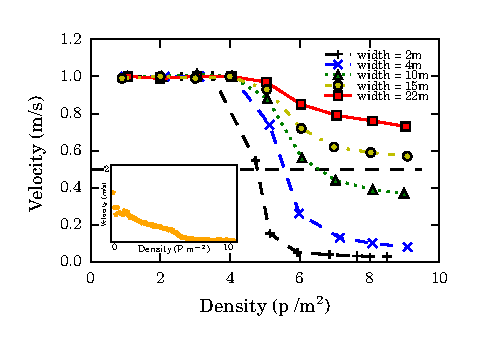
\includegraphics[width=0.5\columnwidth]
{plots/speed-density_vd1_multiple_widths.eps}
\caption{\label{fundamental_diagram_speed} Mean speed ($V$) as a function of the density ($\rho$) for different widths. Initially, 
pedestrians were randomly distributed along the corridor. The measurements were taken in the middle
of the corridor once the system reached the stationary state (see Fig.\ref{corridor}). The length of the corridor 
was 28~m in all cases (with periodic boundary conditions in the \textit{x} direction).}
\end{figure}

We may summarize our first results as follows. We were able to validate the seminal SFM for narrow corridors through the fundamental diagram. However, the SFM (in its current version) disagrees with experimental data as the corridors widen. We will focus in the next Section on the velocity profile in order to investigate this discrepancy. 

\subsection{\label{velocity_profile} Velocity profile}

As we mentioned in Section \ref{fundamental_diagram}, when the density is low, pedestrians achieve the desired velocity ($v=v_d=1$~m/s). Since the results of the previous Section only hold for the area located in the middle of the corridor (see Fig.\ref{corridor}), we want to shed some light and understand what is happening across the entire corridor.\\

Fig.~\ref{speed-profile-w22} shows the velocity profile (velocity vs. \textit{y}-location) of the pedestrians across the corridor (see caption for details). We can see that low-density situations lead to a cruising velocity profile $v=v_d$. This is valid for every location in the corridor (not only the center as was previously noticed in Section \ref{fundamental_diagram}). For higher densities, the velocity profile turns into a parabola-like function. This shape resembles the usual velocity profile for laminar flow in a viscous fluid, where the velocity increases toward the center of a tube. In our case, pedestrians near the walls are the ones with the lower velocity. The velocity increases when departing from the wall until it reaches the maximum at the center of the corridor. This behavior suggests that the wall friction on the pedestrians, is playing a relevant role on the velocity distribution.\\

\begin{figure}[htbp!]
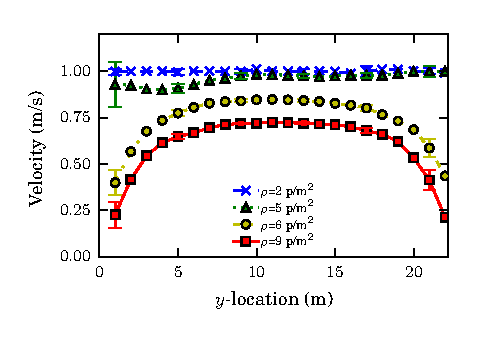
\includegraphics[width=0.5\columnwidth]
{plots/v_y_width22_k24.eps}
\caption{\label{speed-profile-w22} Mean velocity profile (velocity vs \textit{y}-position) for different densities (see the inserted legend). The simulated corridor was 28~m length. Pedestrians walk from left to right with periodic boundary condition in the \textit{x}-direction. Initially, pedestrians were randomly distributed, the corridor width was $w = 22~$m for all the cases. The bin size was 1~m.}
\end{figure}

Fig.~\ref{speed-profile-multi_width} shows the velocity profile for different widths. The horizontal axis of the plot corresponds to the $y$-location normalized by the width of the corridor. The density chosen was $\rho = 6$ since we wanted to study a situation in which pedestrians slow down. Recall that when $\rho<5$, collisions between pedestrians are not relevant (within the SFM). We can see that the lowest velocities occur in the regions near the walls. Additionally, there is a clear relation between $v_{max}$ and the corridor width. That is, the wider the corridor, the higher the maximum reached velocity.\\


\begin{figure}[htbp!]
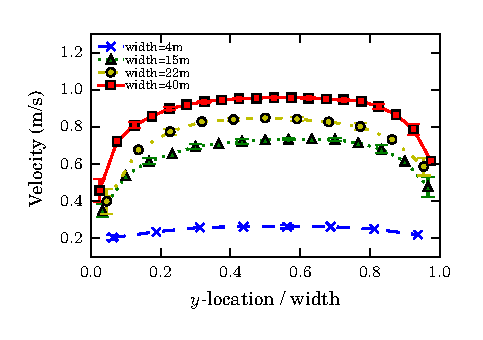
\includegraphics[width=0.5\columnwidth]
{plots/v_y_multi_width.eps}
\caption{\label{speed-profile-multi_width} Velocity profile (velocity vs $y$-position) for different corridors width (see legend for the corresponding widths). The simulated corridor was 28~m length. Pedestrians walk from left to right with periodic boundary condition in the $x$-direction. Initially, pedestrians were randomly distributed, the density was $\rho = 6$ in all the cases (high density regime). The bin size was 1~m except for $w=4$~m since the bin was 0.5~m.}
\end{figure}


Fig.~\ref{speed-profile-width-normaliz} exhibits the scaled velocity profile. The horizontal axis is normalized by the corresponding corridor width (just like in Fig.~\ref{speed-profile-multi_width}). Now, the vertical axis is normalized by the maximum velocity ($v_{max}$) corresponding to each data set. Filled markers correspond density $\rho=9$, while empty markers correspond to $\rho=6$. Notice that all the data follow the same  pattern, suggesting that the velocity profile exhibits a somewhat fundamental behavior, regardless the scale of the corridor (and the density). Hence, the velocity growth rate from the wall towards the center of the corridor, is the same in spite of the size of the corridor width and the density. \\

\begin{figure}[htbp!]
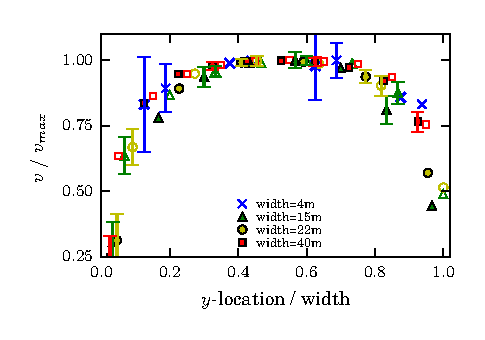
\includegraphics[width=0.5\columnwidth]
{plots/v_y_multi_width_normaliz.eps}
\caption{\label{speed-profile-width-normaliz} Scaled velocity profile (normalized velocity) vs. $y$-location for different corridors width (see legend for the corresponding widths) and two different densities. Empty markers correspond to $\rho=6$ while filled markers correspond to  $\rho=9$. The simulated corridor was 28~m length. Pedestrians walk from left to right with periodic boundary condition in the $x$-direction. Initially, pedestrians were randomly distributed. The horizontal axis is normalized by the corridor width, the vertical axis is normalized by the maximum velocity reached in each case.  The bin size was 1~m for all cases except for $w=4$~m since the bin was 0.5~m.}
\end{figure}

In summary, the scaled velocity profile (see Fig.~\ref{speed-profile-width-normaliz}) does not report any relevant difference as the corridor widens (withing the high density regime). This suggests that the pedestrian dynamics remain essentially the same. The maximum attainable velocity ($v_{max}$), however, seems to be a sensible parameter with respect to the flux.  The narrow corridors attain lower values of $v_{max}$ and thus lower flux. We may expect the flow not to increase if $v_{max}$ remains low enough along the explored density range.\\


We may hypothesize that the friction force is somehow the key factor in the
flow reduction, as reported in the experimental fundamental diagram. This hypothesis further inspired us to analyze the role of the friction coefficient in a simple model for the corridor (see Appendix \ref{appendix_2}). 

\subsection{Work done by friction force}

In the previous Section we studied the velocity profiles for different corridors as a function of density. Here we present the spacial distribution of the work done by the friction force. Only the pedestrian-pedestrian friction was computed.
The work on each pedestrian $i$ was numerically obtained through the integration Trapezoidal rule (according to Ec.~\ref{ec-trapezoidal}). The integration time step was $\Delta t = 0.05$~s. 

\begin{equation}
W^{(i)}(t) \simeq \left [ \vec{f}^{(i)}(t+\Delta t) + \vec{f}^{(i)}(t)  \right ]\cdot \frac{\Delta \vec{x}}{2} \label{ec-trapezoidal}
\end{equation}

Once the work on every pedestrian is calculated, we proceed to bin the corridor into a squared grid of 1~m$\times$1~m cells in order to associate the work values with the corresponding spacial location. Fig.~\ref{abswg} shows three color maps of the absolute value of the work done by the friction force. The horizontal and vertical axis represent the $x$-location and $y$-location of the corridor respectively. The color map associates higher work values with red colors and lower work for blue colors. The walls are located at $y=0$ and $y=w$ (bottom and top of each figure). Fig.~\ref{abswg_width10} corresponds to a 10 m width corridor, Fig.~\ref{abswg_width15} corresponds to a 15 m width corridor and Fig.~\ref{abswg_width22} corresponds to a 22 m width corridor.\\

In the three figures we observe a similar pattern: the regions near the walls (bottom and top) are the most dissipative ones. The center of the corridor is though not a very dissipative region. Furthermore, the work seems to increase with the corridor width. This occurs because the relative velocity between pedestrians is greater in the wide corridors than in narrow ones. This can be checked by comparing the slopes between parabolas in Fig.~\ref{speed-profile-multi_width}. As can be seen there, the wider the corridor, the greater the slope (corresponding to locations near the wall).\\

Recall from Eq.(\ref{granular}), that the friction force depends on the compression and the relative velocity among pedestrians. The compression levels remain the same in the three cases since the compression only depends on the density (which is fix at $\rho=6$ for the three color maps). Thus, the differences between Figs.~\ref{abswg_width10}, \ref{abswg_width15} and \ref{abswg_width22} can only explained by the increment of the relative velocity between individuals. \\

\begin{figure}[!htbp]
    \subfloat[]{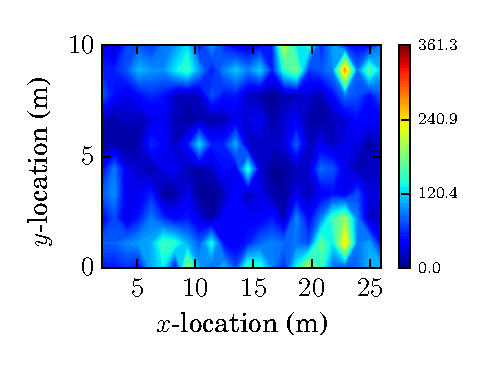
\includegraphics[width=0.5\columnwidth]{plots/abswg_width10.eps}\label{abswg_width10}}\\ 
    \subfloat[]{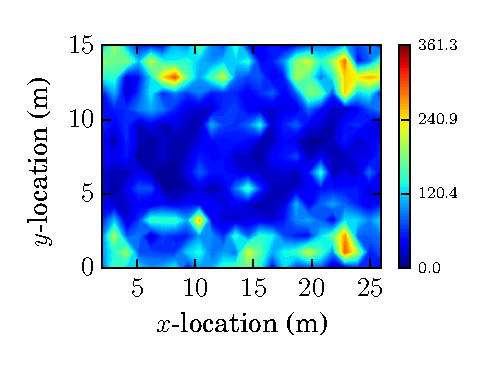
\includegraphics[width=0.5\columnwidth]{plots/abswg_width15.eps}\label{abswg_width15}}\\
    \subfloat[]{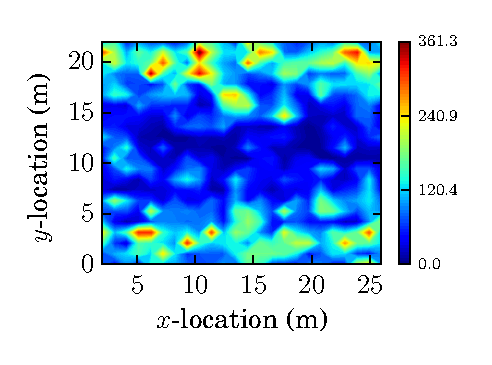
\includegraphics[width=0.5\columnwidth]{plots/abswg_width22.eps}\label{abswg_width22}}\
\caption[width=0.47\columnwidth] {Color map for the absolute value of the work done by the friction. The density chose was $\rho=6$. (a) Corresponds to $w=$10~m (b) $w=$15~m and (c) $w=$22~m. The axis represent the location in the corridor ($x$ and $y$). The scale bar on the right is expressed in Joule units. The work was numerically integrated following the Trapezoidal rule with $\Delta t =0.05$~s. The pedestrians desired velocity was $v_d = 1$~m/s. The contour lines were computed on a square grid of 1m$\times$~1m and then splined to get smoother curves.} 
\label{abswg}
\end{figure}

The above observations drive the following conclusion. The maximum attainable velocity $v_{max}$ accomplishes a maximum velocity slope (with its associated friction dissipation). Both the friction with the walls and the friction between the pedestrians appear as relevant magnitudes for properly slowing down the crowd velocity, in order to fit the experimental data. Appendix \ref{appendix_2} supports this assertion with a simple example.  

\subsection{Friction modification}

As already mentioned, the results shown so far indicate that friction may be the key magnitude for fitting the fundamental diagram into the experimental data. We want to make clear that fitting the experimental data means mimicking (qualitatively) the congested regime reported by different authors (including the Jamaraat study in Ref.~\cite{helbing3}) for corridors as width as 22~m. The seminal version of the Social Force Model proposes the same friction coefficient for the pedestrian-pedestrian interaction and the pedestrian-wall interaction. The proposed value was $\kappa = 2.4\times10^{5}$. This value is widely used in many studies.  \\

We tested the friction coefficient modification in Appendix \ref{appendix_2} and we found that the fundamental diagram experiences a qualitatively change when the friction coefficient $\kappa$ is varied. We further performed numerical simulations in the context of the SFM. We call $\kappa_i$ as the friction coefficient of the pedestrian-pedestrian interaction and $\kappa_w$ as the friction coefficient of the pedestrian-wall interaction. Fig.~\ref{fgmodified-w22} shows the flow vs density for different values of $\kappa_i$ and $\kappa_w$.\\

The triangular symbols in Fig.~\ref{fgmodified-w22} correspond to the increase in one order of magnitude of the wall friction (now $\kappa_w = 2.4\times10^{6}$), leaving the pedestrian-pedestrian friction unchanged (\textit{i.e.}, $\kappa_i = 2.4\times10^{5}$). We can see that the flow reduces a little bit, but this is not enough to change significantly the congested regime. \\

The circles in Fig.~\ref{fgmodified-w22} correspond to a modification of the friction between pedestrians without changing the value of the wall friction. We increased the pedestrian-pedestrian friction by a factor of ten ($\kappa_i = 2.4\times10^{6}$). Here we see a significant reduction of the flow. The qualitative behavior resembles the fundamental diagram reported by Helbing \textit{et al}. with a well defined congested regime for the greatest densities.\\

We also tested the case were both friction coefficients surpass ten times the value of the original model (now $\kappa_w = \kappa_i = 2.4\times10^{6}$). The squared symbols represent this scenario. As expected, the flow reduces significantly respect the original case (cross symbol). Interestingly, the reduction of the flow is more than the reduction due to the increment of $\kappa_i$ plus the reduction of the flow due to $\kappa_w$. This behavior is indicative that the superposition principle does not hold in this system because of the non-linearity of the equation of motion.     \\

This finding allows us to affirm that the friction plays a crucial role in the functional behavior of the fundamental diagram. The increment of both individual-individual friction and wall friction are determinant in order to achieve a congested regime. More specifically, the empirical behavior for the fundamental diagram can be achieved by properly increasing the friction coefficients. In Appendix \ref{appendix_3} we show that the friction modification does not alter already studied behaviors of pedestrian dynamics.\\

Recall that other authors address the ``congested regime problem" by modifying different aspects of the model. Ref.~\cite{parisi2} imposes zero desired velocity once pedestrians are close enough, Ref.~\cite{johansson} increases the relaxation time in order to slow down the net-time headway, and more recently,  Ref.~\cite{kwak} induce the jamming transition by an attraction. Many of these approaches seem to be equivalent. In Appendix \ref{appendix_1} we discuss about how the modification of the relaxation time and the increment of the friction coefficient yield a similar effect, since both affect the same term in the reduced-in-units equation of motion.  The relaxation time, however, also affects the social interactions (see Section \ref{Hypotheses} and Appendix \ref{appendix_1}).   \\

We claim that in real scenarios, a combination of all these factors may be the cause of the marked flow reduction that portray the fundamental diagram. The pedestrians path can be very complex even if it is a simple enclosure (straight corridor) and the target is well defined (unidirectional flow). Beyond the complexities given by the internal motivations of pedestrians, we strongly suggest studying and modeling coefficients of friction between individuals and the friction with the walls. These two parameters have shown to be very important in the pedestrian dynamics and deserve a closer inspection in future research.\\

We want to emphasize that the proposals stated in Refs.~\cite{parisi2,johansson,kwak}  only apply under normal conditions. If a crowd is under high levels of anxiety, pedestrians will neither keep distance between each other, nor will feel the urge to see an ``attraction". Thus, studying the friction coefficients may be a critical factor to properly reproduce the dynamics of a massive evacuation under stress.\\

With all these insights, we can say that the narrow corridors have no drawback in the fitting of the flow vs. density relation because very high velocities are not attainable. This happens because in narrow corridors, the friction of the walls has a lot of ``relative weight" in the overall friction of the system. 
The friction exerted by the walls is fundamental in order to produce the parabolic shape of the velocity profile. The walls provide friction force in the opposite direction to the speed of the individual (drag backwards), since they act like a fixed pedestrian. In other ways, friction between pedestrians can produce either drag forward or drag backwards depending on the the contacting pedestrians velocities (see Eq.~\ref{granular}).\\


\begin{figure}[htbp!]
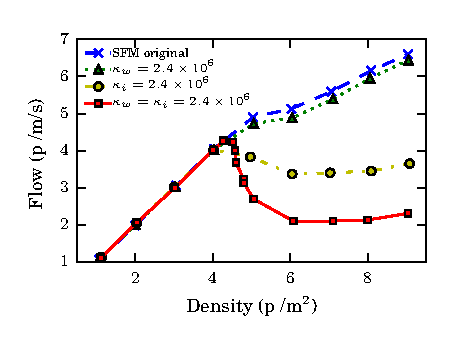
\includegraphics[width=0.5\columnwidth]
{plots/flow-density_pasillo22m_fgmodified_multi.eps}
\caption{\label{fgmodified-w22} Fundamental diagram (flow vs density) for different friction coefficient (see legend for the corresponding values). The simulated corridor was 28~m length. Pedestrians walk from left to right with periodic boundary condition in the $x$-direction. Initially, pedestrians were randomly distributed. For each density, we measure the flow once the system reaches the stationary state.}
\end{figure}

In this subsection we have shown that an adequate modification of the friction coefficients yields a fundamental diagram that follows qualitatively the behavior reported through empirical data (say flow reduction for the highest densities). We have also discussed different approaches proposed by other authors in order to overcome this problem. See Appendix \ref{appendix_1} for a more detailed discussion.\\

\subsection{\label{clusters}Clusters}

Cluster formation is a very important process in pedestrian dynamics. Moreover, is the key process that explains the clogging phenomena in bottleneck evacuations. We analyzed the clustering formation according to the granular cluster definition given in~\ref{granular-cluster}. Fig.~\ref{cluster_distribution} shows the histograms of the cluster size distribution for three different densities, from top to bottom: $\rho=4.5$, $\rho=5$ and $\rho=5.5$. These three
densities are representative for the crossover between
a non-clusterized regime and a unique “giant” cluster
regime. We studied two situations for each density: the
seminal SFM on left hand side plots, and the enhanced
friction situation on the right hand side plots (see
caption for details).\\

We found two unexpected results. Increasing the density produces bigger size clusters until the size distribution suddenly switches to a bimodal distribution (compare \ref{size_distribution_w22_density5} with \ref{size_distribution_w22_density5_5} and \ref{size_distribution_w22_density4.5_kx10} with \ref{size_distribution_w22_density5_kx10}). Once
this phenomenon occurs, any of two possibilities may
appear: the pedestrian belongs to a small cluster (out
of many caged in the crowd) or he (she) belongs to the
giant cluster (with a size comparable to the entire crowd).\\

We also observed that this phenomenon is controlled by the friction. For higher frictions, the crossover to the bimodal distribution occurs at lower densities (see Fig.~\ref{size_distribution_w22_density5} and Fig.~\ref{size_distribution_w22_density5_kx10}). Despite the fact that both correspond to the same density, Fig.~\ref{size_distribution_w22_density5_kx10} already attained the bimodal distribution since the friction force is ten times greater than in Fig.~\ref{size_distribution_w22_density5}. This peculiar phenomenon
occurs because in an enhanced friction scenario the
individuals find it harder to detach from each other. On
the opposite, when the friction is weak, the individuals
detach themselves more easily, leading to a situation
where large clusters are less probable.\\

\begin{figure}[!htbp]
    \subfloat[]{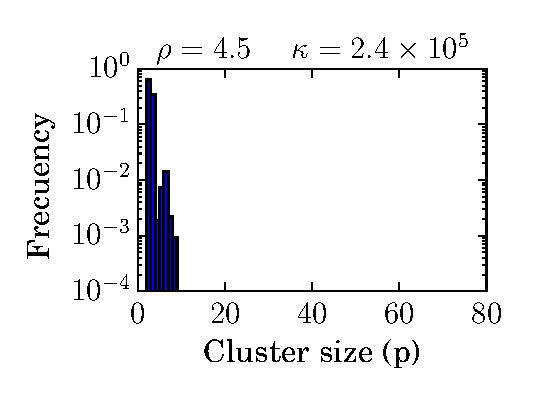
\includegraphics[width=0.40\columnwidth]{plots/size_distribution_w22_density4_5.eps}\label{size_distribution_w22_density4.5}}\ 
    \subfloat[]{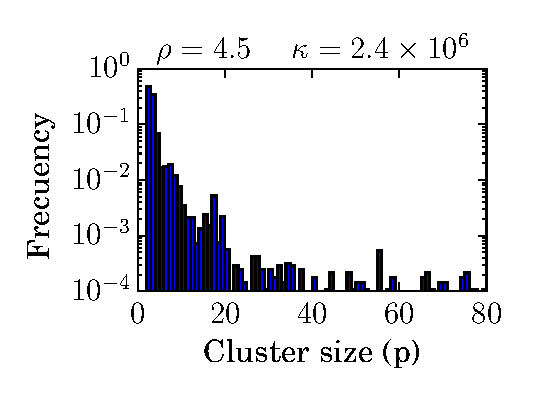
\includegraphics[width=0.40\columnwidth]{plots/size_distribution_w22_density4_5_kx10.eps}\label{size_distribution_w22_density4.5_kx10}}\\
    \subfloat[]{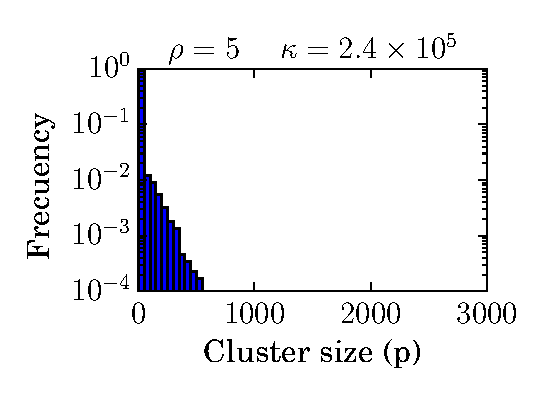
\includegraphics[width=0.40\columnwidth]{plots/size_distribution_w22_density5.eps}\label{size_distribution_w22_density5}}\
    \subfloat[]{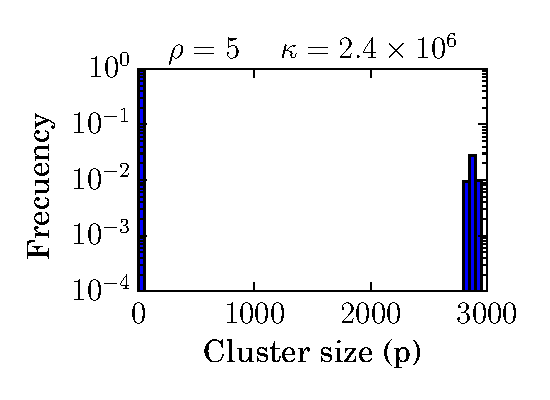
\includegraphics[width=0.40\columnwidth]{plots/size_distribution_w22_density5_kx10.eps}\label{size_distribution_w22_density5_kx10}}\\
    \subfloat[]{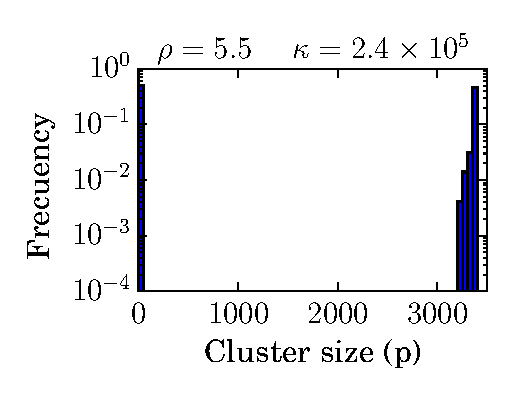
\includegraphics[width=0.40\columnwidth]{plots/size_distribution_w22_density5_5.eps}\label{size_distribution_w22_density5_5}}\
    \subfloat[]{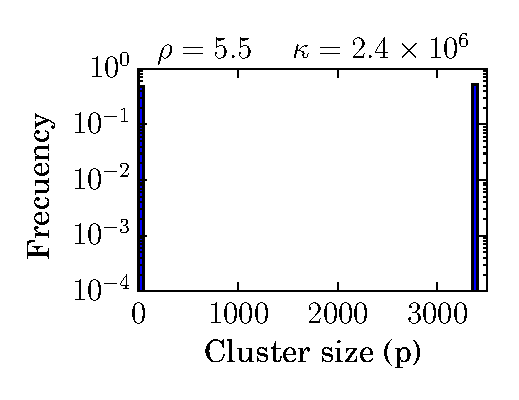
\includegraphics[width=0.40\columnwidth]{plots/size_distribution_w22_density5_5_kx10.eps}\label{size_distribution_w22_density5_5_kx10}}
\caption[width=0.47\columnwidth]{Cluster size distribution for six different scenarios. (a) SFM friction parameters and $\rho=4.5$, the bin size is 1 p (b) friction parameters increased by a factor of ten and $\rho=4.5$, the bin size is 1 p (c) SFM friction parameters and $\rho=5$, the bin size is 50 p (d) friction parameters increased by a factor of ten and $\rho=5$, the bin size is 50 p (e) SFM friction parameters and $\rho=5.5$, the bin size is 50 p (f) friction parameters increased by a factor of ten and $\rho=5.5$, the bin size is 50 p.}
\label{cluster_distribution}
\end{figure}

To get a better view of this phenomenon, we represent in Fig.~\ref{fic} the fraction of clustered individual as a function of the density for four different situations in which we only changed the friction coefficients. The fraction of clustered individuals is defined as the amount of pedestrians that belong to a cluster (of two or more individuals) over the total number pedestrians in the corridor. 
We can see that there is a transition from a non-clustered crowd to a full-clustered crowd. This transition occurs in a very narrow range of densities, causing the cluster formation process to occur between $4.4<\rho<5.3$. When the friction coefficient is enhanced, the transition takes place at a lower density threshold. This result is in complete agreement with the histograms shown in Fig.~\ref{cluster_distribution}, confirming the fact that friction promotes the formation of clusters.\\

As expected, the transition sharpens when both $\kappa_i$ and $\kappa_w$ are increased (squared symbol in Fig.~\ref{fic}). However, the fraction of clustered individuals is always greater than in the original SFM when just one of the
two coefficients is increased. Notice that there is not a big difference between the modification of $\kappa_i$ and the modification of $\kappa_w$. This suggests that it does not really matter if the clusterization starts at the areas close to the walls or in the middle of the crowd.\\


\begin{figure}[htbp!]
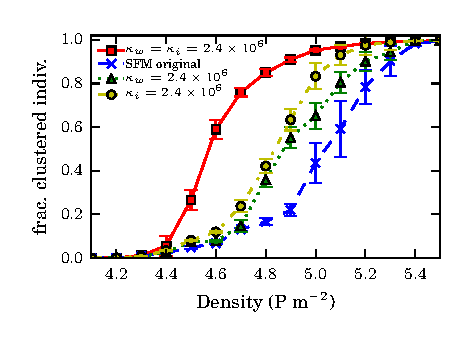
\includegraphics[width=0.5\columnwidth]
{plots/fracc_clusteriz_vs_density.eps}
\caption{\label{fic} Fraction of clustered individuals as a function of the density. Squared symbols correspond to $\kappa_w=\kappa_i=2.4\times 10^6$, circles to $\kappa_i=2.4\times 10^6$ and $\kappa_w=2.4\times 10^5$, triangles to to $\kappa_i=2.4\times 10^5$ and $\kappa_w=2.4\times 10^6$ and crosses to the coefficients of the original Social Force model ($\kappa_i=2.4\times 10^5$ and $\kappa_w=2.4\times 10^5$). The pedestrians walk across a corridor with $v_d=1$m/s. The measurements were recorded every 0.5~s once the system reached the stationary state. The values corresponding to the fraction of clustered individuals were averaged over 170~s. The cluster cutoff distance was 0.46~m (equivalent to the shoulder width of the pedestrians).}
\end{figure}

Two main conclusions can be outlined from the above
results. The friction coefficients between the pedestrians
(and with the walls) appear as decisive parameters
with respect to the crossover between the freely moving
regime and the slow down regime. The precise (density) threshold between both regimes will actually depend on
the friction coefficients, since these control the efforts
required by the pedestrians to detach from each other.
Above this threshold (say, at high densities) the whole
crowd slows down, since the pedestrians appear mostly
clustered or ``caged" in a clustered environment.\\

